\documentclass[italian]{article}
\usepackage[T1]{fontenc}
\usepackage[utf8]{inputenc}
\usepackage{lmodern}
\usepackage{hyperref}
\usepackage[a4paper,top=3cm,bottom=3cm,left=2.5cm,right=2.5cm]{geometry}
\usepackage[italian]{babel}
\usepackage{listings} %Per inserire codice
\usepackage[usenames]{color} %Per permettere la colorazione dei caratteri 
%Define the listing package
\usepackage{listings} %code highlighter
\usepackage{color} %use color
\usepackage{graphicx}
\graphicspath{ {./images/} }
\definecolor{mygreen}{rgb}{0,0.6,0}
\definecolor{mygray}{rgb}{0.5,0.5,0.5}
\definecolor{mymauve}{rgb}{0.58,0,0.82}

%Customize a bit the look
\lstset{ %
	backgroundcolor=\color{white}, % choose the background color; you must add \usepackage{color} or \usepackage{xcolor}
	basicstyle=\footnotesize, % the size of the fonts that are used for the code
	breakatwhitespace=false, % sets if automatic breaks should only happen at whitespace
	breaklines=true, % sets automatic line breaking
	captionpos=b, % sets the caption-position to bottom
	commentstyle=\color{mygreen}, % comment style
	deletekeywords={...}, % if you want to delete keywords from the given language
	escapeinside={\%*}{*)}, % if you want to add LaTeX within your code
	extendedchars=true, % lets you use non-ASCII characters; for 8-bits encodings only, does not work with UTF-8
	frame=single, % adds a frame around the code
	keepspaces=true, % keeps spaces in text, useful for keeping indentation of code (possibly needs columns=flexible)
	keywordstyle=\color{blue}, % keyword style
	% language=Octave, % the language of the code
	morekeywords={*,...}, % if you want to add more keywords to the set
	numbers=left, % where to put the line-numbers; possible values are (none, left, right)
	numbersep=5pt, % how far the line-numbers are from the code
	numberstyle=\tiny\color{mygray}, % the style that is used for the line-numbers
	rulecolor=\color{black}, % if not set, the frame-color may be changed on line-breaks within not-black text (e.g. comments (green here))
	showspaces=false, % show spaces everywhere adding particular underscores; it overrides 'showstringspaces'
	showstringspaces=false, % underline spaces within strings only
	showtabs=false, % show tabs within strings adding particular underscores
	stepnumber=1, % the step between two line-numbers. If it's 1, each line will be numbered
	stringstyle=\color{mymauve}, % string literal style
	tabsize=2, % sets default tabsize to 2 spaces
	title=\lstname % show the filename of files included with \lstinputlisting; also try caption instead of title
}
%END of listing package%

\definecolor{darkgray}{rgb}{.4,.4,.4}
\definecolor{purple}{rgb}{0.65, 0.12, 0.82}

%define Javascript language
\lstdefinelanguage{JavaScript}{
	keywords={typeof, new, true, false, catch, function, return, null, catch, switch, var, if, in, while, do, else, case, break},
	keywordstyle=\color{blue}\bfseries,
	ndkeywords={class, export, boolean, throw, implements, import, this},
	ndkeywordstyle=\color{darkgray}\bfseries,
	identifierstyle=\color{black},
	sensitive=false,
	comment=[l]{//},
	morecomment=[s]{/*}{*/},
	commentstyle=\color{purple}\ttfamily,
	stringstyle=\color{red}\ttfamily,
	morestring=[b]',
	morestring=[b]"
}

\lstset{
	language=JavaScript,
	extendedchars=true,
	basicstyle=\footnotesize\ttfamily,
	showstringspaces=false,
	showspaces=false,
	numbers=left,
	numberstyle=\footnotesize,
	numbersep=9pt,
	tabsize=2,
	breaklines=true,
	showtabs=false,
	captionpos=b
}
\author{
	Daniele Rigon - 857319 \\
}

\begin{document}
\title{Tesi - Payment Request API}
\maketitle

\tableofcontents
\pagebreak

\section{Overview}
I service worker agiscono essenzialmente come server proxy che si trovano tra le applicazioni Web, il browser e la rete (se disponibile). Sono pensati, tra le altre cose, per consentire la creazione di esperienze offline efficaci, intercettare le richieste di rete e intraprendere azioni appropriate in base al fatto che la rete sia disponibile e aggiornare le risorse che risiedono sul server. Consentiranno inoltre l'accesso alle notifiche push e alle API di sincronizzazione in background.

Un problema prioritario con cui gli utenti Web hanno sofferto per anni è la perdita di connettività. La migliore app web al mondo fornirà un'esperienza utente terribile se non puoi scaricarlo. Ci sono stati vari tentativi di creare tecnologie per risolvere questo problema, come mostra la nostra pagina Offline , e alcuni dei problemi sono stati risolti. Ma il problema principale è che non esiste ancora un buon meccanismo di controllo generale per il caching delle risorse e le richieste di rete personalizzate. 

Il precedente tentativo - AppCache - sembrava essere una buona idea perché ti permetteva di specificare le risorse in modo molto semplice. Tuttavia, ha fatto molte supposizioni su quello che stavi cercando di fare e poi si è rotto in modo orribile quando la tua app non ha seguito esattamente queste ipotesi

I lavoratori del servizio dovrebbero finalmente risolvere questi problemi. La sintassi del service worker è più complessa di quella di AppCache, ma il compromesso è che è possibile utilizzare JavaScript per controllare i comportamenti impliciti di AppCache con un grado di granularità fine, che consente di gestire questo problema e molti altri ancora. Utilizzando un operatore del servizio, puoi facilmente impostare un'app per utilizzare prima le risorse memorizzate nella cache, fornendo così un'esperienza predefinita anche offline, prima di ottenere più dati dalla rete (comunemente nota come Prima non in linea ). Questo è già disponibile con le app native, che è uno dei motivi principali per cui le app native vengono spesso scelte su app web.

\section{Concetti e utilizzo del service worker}
Un lavoratore di servizio è un lavoratore guidato da eventi registrato su un'origine e un percorso. Prende la forma di un file JavaScript in grado di controllare la pagina web / sito a cui è associato, intercettare e modificare le richieste di navigazione e risorse e memorizzare le risorse in modo granulare per darti il controllo completo su come si comporta la tua app in determinate situazioni , (il più ovvio è quando la rete non è disponibile.)

Un addetto al servizio viene eseguito in un contesto di lavoro: non ha quindi accesso a DOM e viene eseguito su un thread diverso dal JavaScript principale che alimenta la tua app, quindi non si blocca. È progettato per essere completamente asincrono; di conseguenza, le API come XHR sincrono e localStorage non possono essere utilizzate all'interno di un operatore di servizio.

Gli addetti all'assistenza funzionano solo su HTTPS, per motivi di sicurezza. Avendo modificato le richieste di rete, gli attacchi spalancati agli uomini nel mezzo sarebbero davvero pessimi. In Firefox, anche le API di Service Worker sono nascoste e non possono essere utilizzate quando l'utente è in modalità di navigazione privata .

\section{Registrazione}
Un addetto all'assistenza viene prima registrato utilizzando il ServiceWorkerContainer.register()metodo. In caso di esito positivo, l'addetto all'assistenza verrà scaricato sul client e tenterà l'installazione / attivazione (vedere di seguito) per gli URL a cui l'utente ha avuto accesso all'interno dell'intera origine o all'interno di un sottoinsieme specificato dall'utente.

\section{Impostare i service worker}
Molte funzionalità dei lavoratori del servizio ora sono abilitate di default nelle versioni più recenti dei browser di supporto. Se tuttavia trovi che il codice demo non funziona nelle tue versioni installate, potresti dover abilitare un pref:
\begin{itemize}
\item Firefox: vai su \url{about:config} e imposta  dom.serviceWorkers.enabled su true; riavvia il browser.
\item Chrome : vai a  \url{chrome://flags} e accendi  experimental-web-platform-features; riavvia browser
\item Opera : vai a \url{opera://flags} e attiva  Support for ServiceWorker; riavvia il browser.
\item Microsoft Edge : vai a  \url{about:flags} e spunta  Enable service workers; riavvia il browser.
\end{itemize}
Dovrai anche servire il tuo codice tramite HTTPS: gli addetti all'assistenza sono costretti a utilizzare HTTPS per motivi di sicurezza. GitHub è quindi un buon posto per ospitare esperimenti, in quanto supporta HTTPS. Al fine di facilitare lo sviluppo locale,  localhost è considerato un'origine sicura anche dai browser.


\subsection{Scarica, installa e attiva}
A questo punto, il tuo operatore di servizio osserverà il seguente ciclo di vita:
\begin{itemize}
\item Scaricare
\item Installare
\item Attivare
\end{itemize}
L'addetto all'assistenza viene scaricato immediatamente quando un utente accede per la prima volta a un sito / una pagina controllata dal lavoratore.

Successivamente, viene scaricato ogni 24 ore circa. Esso può essere scaricato più di frequente, ma deve essere scaricato ogni 24 ore per impedire l'esecuzione di cattivi da essere fastidioso per troppo tempo.

L'installazione viene tentata quando il file scaricato viene trovato nuovo - diverso da un lavoratore del servizio esistente (confrontato in termini di byte) o il primo operatore di servizio rilevato per questa pagina / sito.

Se questa è la prima volta che un operatore di servizio viene reso disponibile, viene tentata l'installazione, quindi, dopo un'installazione corretta, viene attivata.

Se è disponibile un operatore di servizio esistente, la nuova versione viene installata in background, ma non ancora attivata - a questo punto viene chiamata l' operatore in attesa . Si attiva solo quando non ci sono più pagine caricate che stanno ancora utilizzando il vecchio servizio di assistenza. Non appena non ci sono più pagine da caricare, il nuovo lavoratore di servizio si attiva (diventando il lavoratore attivo ). L'attivazione può avvenire prima utilizzando ServiceWorkerGlobalScope.skipWaiting()e le pagine esistenti possono essere richieste dal lavoratore attivo che utilizza Clients.claim().

Puoi ascoltare per il InstallEvent; un'azione standard è quella di preparare il tuo operatore di servizio all'utilizzo quando questo si attiva, ad esempio creando una cache utilizzando l'API di archiviazione integrata e inserendo risorse al suo interno che ti serviranno per eseguire la tua app offline.

C'è anche un activateevento. Il punto in cui questo evento si attiva è generalmente un buon momento per ripulire le vecchie cache e altre cose associate alla versione precedente del proprio addetto all'assistenza.

Il tuo addetto all'assistenza può rispondere alle richieste utilizzando l' FetchEventevento. È possibile modificare la risposta a queste richieste nel modo desiderato, utilizzando il FetchEvent.respondWithmetodo.

\section{Casi d'uso}
Gli addetti all'assistenza sono anche destinati a essere utilizzati per cose come:
\begin{itemize}
\item Sincronizzazione dei dati in background
\item Rispondendo alle richieste di risorse da altre origini
\item Ricezione di aggiornamenti centralizzati a dati costosi da calcolare come la geolocalizzazione o il giroscopio, in modo che più pagine possano utilizzare un set di dati
\item Compilazione lato client e gestione delle dipendenze di CoffeeScript, meno, moduli CJS / AMD, ecc. Per scopi di sviluppo
\item Ganci per servizi in background
\item Modelli personalizzati basati su determinati pattern URL
\item Miglioramenti delle prestazioni, ad esempio prelettura delle risorse che l'utente probabilmente avrà bisogno nel prossimo futuro, come le prossime foto in un album fotografico.
\end{itemize}
In futuro, gli addetti all'assistenza saranno in grado di fare una serie di altre cose utili per la piattaforma web che la avvicineranno alla praticabilità delle app native. È interessante notare che altre specifiche possono e cominceranno a utilizzare il contesto di servizio, ad esempio:
\begin{itemize}
\item Sincronizzazione in background : avvia un operatore di servizio anche quando nessun utente si trova sul sito, quindi le cache possono essere aggiornate, ecc.
\item Reagire per inviare messaggi : Avviate un addetto all'assistenza per inviare agli utenti un messaggio per comunicare loro che sono disponibili nuovi contenuti.
\item Reagendo a un'ora e data particolari
\item Entrando in una geo-recinzione
\end{itemize}

\section{Architettura di base}
Con gli operatori di servizio, i seguenti passaggi vengono generalmente osservati per l'impostazione di base:
\begin{itemize}
\item L'URL dell'operatore di servizio viene recuperato e registrato tramite serviceWorkerContainer.register().
\item In caso di esito positivo, l'addetto all'assistenza viene eseguito in a ServiceWorkerGlobalScope; questo è fondamentalmente un tipo speciale di contesto di lavoro, che scappa dal thread di esecuzione dello script principale, senza accesso DOM.
\item Il lavoratore del servizio è ora pronto per elaborare gli eventi.
\item L'installazione del lavoratore viene tentata quando si accede successivamente alle pagine controllate dal personale dell'assistenza. Un evento di installazione è sempre il primo inviato a un operatore del servizio (questo può essere utilizzato per avviare il processo di compilazione di un IndexedDB e la memorizzazione nella cache delle risorse del sito). Questo è in realtà lo stesso tipo di procedura di installazione di un'applicazione nativa o di Firefox OS, rendendo tutto disponibile per l'uso offline.
\item Al termine del oninstallgestore, il lavoratore del servizio è considerato installato.
\item Il prossimo è l'attivazione. Quando il worker del servizio è installato, riceve quindi un evento di attivazione. L'uso principale di onactivateè per la pulizia delle risorse utilizzate nelle versioni precedenti di uno script di servizio.
\item L'addetto all'assistenza ora controllerà le pagine, ma solo quelle aperte dopo il register()successo. cioè un documento inizia la vita con o senza un operatore del servizio e lo mantiene per tutta la sua durata. Quindi i documenti dovranno essere ricaricati per essere effettivamente controllati.
\end{itemize}
\begin{figure}
	\centering
	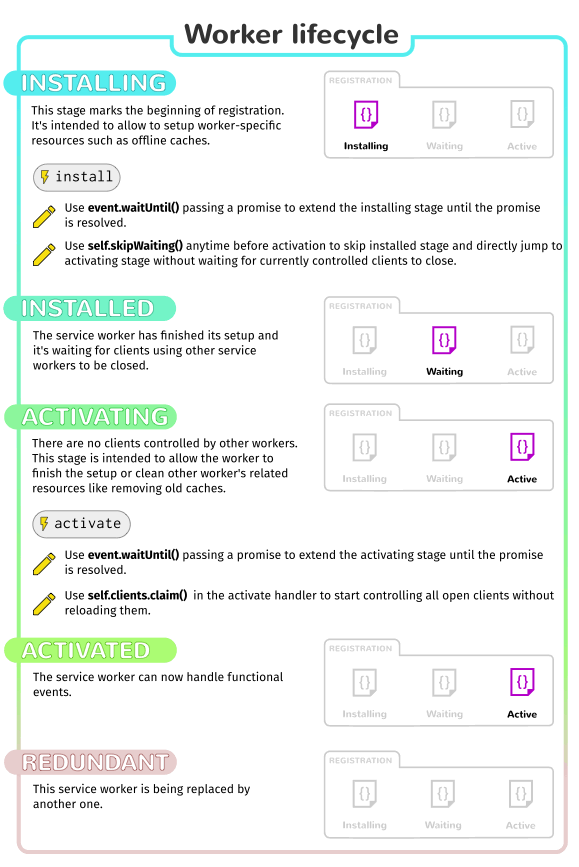
\includegraphics[width=1\linewidth]{SwLifecycle}
	\caption{Ciclo di vita del Service Worker}
	\label{fig:Ciclo di vita del Service Worker}
\end{figure}


\section{Specifiche}
\subsection{Metodi}
\subsubsection{Cache}
Rappresenta le coppie di archiviazione Request/ Responseoggetto che vengono memorizzate nella cache come parte del ServiceWorkerciclo di vita.
\subsubsection{CacheStorage}
Rappresenta la memoria per gli Cacheoggetti. Fornisce una directory principale di tutte le cache nominate a cui ServiceWorkerpuò accedere e mantiene una mappatura dei nomi delle stringhe agli Cacheoggetti corrispondenti .
\subsubsection{Client}
Rappresenta l'ambito di un client worker del servizio. Un client worker del servizio è un documento in un contesto browser o a SharedWorker, che è controllato da un lavoratore attivo.
\subsubsection{Clients}
Rappresenta un contenitore per un elenco di Clientoggetti; il modo principale per accedere ai client worker del servizio attivo all'origine corrente.
\subsubsection{ExtendableEvent}
Estende la durata installe gli activateeventi inviati sul ServiceWorkerGlobalScope, come parte del ciclo di vita del lavoratore del servizio. Ciò garantisce che nessun evento funzionale (come FetchEvent) venga inviato a ServiceWorker, fino a quando non aggiorna gli schemi di database, e cancella le voci obsolete della cache, ecc.
\subsubsection{ExtendableMessageEvent}
L'oggetto evento di un messageevento attivato su un operatore di servizio (quando un messaggio di canale viene ricevuto ServiceWorkerGlobalScopeda un altro contesto) estende la durata di tali eventi.
\subsubsection{FetchEvent}
Il parametro passato al ServiceWorkerGlobalScope.onfetchgestore, FetchEventrappresenta un'azione di recupero che viene inviata su ServiceWorkerGlobalScopea ServiceWorker. Contiene informazioni sulla richiesta e sulla risposta risultante e fornisce il FetchEvent.respondWith()metodo, che ci consente di fornire una risposta arbitraria alla pagina controllata.
\subsubsection{InstallEvent}
Il parametro passato al oninstallgestore, l' InstallEventinterfaccia rappresenta un'azione di installazione che viene inviata su ServiceWorkerGlobalScopea ServiceWorker. Fin da bambino ExtendableEvent, garantisce che eventi funzionali come quelli FetchEventnon vengano inviati durante l'installazione.
\subsubsection{NavigationPreloadManager}
Fornisce metodi per la gestione del pre-caricamento delle risorse con un operatore di servizio.
\subsubsection{Navigator.serviceWorker}
Restituisce un ServiceWorkerContaineroggetto, che fornisce accesso alla registrazione, rimozione, aggiornamento e comunicazione con gli ServiceWorkeroggetti per il documento associato .
\subsubsection{NotificationEvent}
Il parametro passato al onnotificationclickgestore, l' NotificationEventinterfaccia rappresenta un evento di notifica che viene inviato su ServiceWorkerGlobalScopea ServiceWorker.
\subsubsection{ServiceWorker}
Rappresenta un addetto all'assistenza. È possibile associare più contesti di navigazione (ad es. Pagine, lavoratori, ecc.) Allo stesso ServiceWorkeroggetto.
\subsubsection{ServiceWorkerContainer}
Fornisce un oggetto che rappresenta il lavoratore del servizio come un'unità generale nell'ecosistema di rete, incluse le strutture per registrare, annullare la registrazione e aggiornare i lavoratori del servizio e accedere allo stato dei lavoratori dei servizi e alle loro registrazioni.
\subsubsection{ServiceWorkerGlobalScope}
Rappresenta il contesto di esecuzione globale di un operatore di servizio.
\subsubsection{ServiceWorkerMessageEvent}
Rappresenta un messaggio inviato a ServiceWorkerGlobalScope. Nota che questa interfaccia è deprecata nei browser moderni. I messaggi di service worker ora utilizzano l' MessageEventinterfaccia, per coerenza con le altre funzionalità di messaggistica web.
\subsubsection{ServiceWorkerRegistration}
Rappresenta una registrazione di lavoratore di servizio.
\subsubsection{ServiceWorkerState}
Associata al suo ServiceWorkerstato.
\subsubsection{SyncEvent}
L'interfaccia SyncEvent rappresenta un'azione di sincronizzazione inviata su ServiceWorkerGlobalScopeun ServiceWorker.
\subsubsection{SyncManager}
Fornisce un'interfaccia per la registrazione e l'elenco delle registrazioni di sincronizzazione.
\subsubsection{WindowClient}
Rappresenta l'ambito di un client worker del servizio che è un documento in un contesto browser, controllato da un lavoratore attivo. Questo è un tipo speciale di Clientoggetto, con alcuni metodi e proprietà aggiuntivi disponibili.

\subsection{Promises}
Le promesse sono un ottimo meccanismo per eseguire operazioni asincrone, con il successo che dipende l'una dall'altra. Questo è fondamentale per il modo in cui i lavoratori del servizio lavorano. 

Le promesse possono fare molte cose, ma per ora, tutto quello che dovete sapere è che se qualcosa restituisce una promessa, è possibile collegare .then()fino alla fine e includere i callback al suo interno per il successo, il fallimento, ecc, o è possibile inserire .catch()sul fine se si desidera includere un callback di errore.

Confrontiamo una struttura di callback sincrono tradizionale con il suo equivalente di promessa asincrona.
\begin{itemize}
\item sincrona 
\begin{lstlisting}
	try {
		var value = myFunction();
		console.log(value);
	} catch(err) {
		console.log(err);
	}
\end{lstlisting}
dobbiamo attendere myFunction()l'esecuzione e il ritorno valueprima che possa essere eseguito qualsiasi altro codice
\item  asincrona
\begin{lstlisting}
	myFunction().then(function(value) {
		console.log(value);
	}).catch(function(err) {
			console.log(err);
		});
\end{lstlisting}
myFunction()restituisce una promessa value, quindi il resto del codice può continuare a essere in esecuzione. Quando la promessa si risolve, il codice interno thenverrà eseguito in modo asincrono. 
\end{itemize}
Ora per un esempio reale: cosa accadrebbe se volessimo caricare le immagini in modo dinamico, ma volevamo assicurarci che le immagini fossero caricate prima di provare a visualizzarle? Questa è una cosa standard da voler fare, ma può essere un po 'un dolore. Possiamo usare .onloadsolo per visualizzare l'immagine dopo che è stata caricata, ma per quanto riguarda gli eventi che iniziano a verificarsi prima di iniziare ad ascoltarli? Potremmo provare a aggirare questo usando.complete, ma non è ancora infallibile, e per quanto riguarda le immagini multiple? è ancora sincrono, quindi blocca il thread principale. 

\begin{lstlisting}
	function imgLoad(url) {
		return new Promise(function(resolve, reject) {      
			var request = new XMLHttpRequest();
			request.open('GET', url);
			request.responseType = 'blob';
			
			request.onload = function() {
			if (request.status == 200) {
				resolve(request.response);
			} else {
					reject(Error('Image didn\'t load successfully; error code:' + request.statusText));
				}
		};	
		request.onerror = function() {
			reject(Error('There was a network error.'));
		};	
		request.send();
		});
	}
\end{lstlisting}
Restituiamo una nuova promessa usando il Promise()costruttore, che prende come argomento una funzione di callback con resolvee rejectparametri. Da qualche parte nella funzione, dobbiamo definire cosa accade per la promessa di risolvere con successo o essere respinto - in questo caso restituire uno stato 200 OK o meno - e quindi chiamare resolvesu successo, o rejectin caso di fallimento. Il resto del contenuto di questa funzione è roba XHR abbastanza standard, quindi per ora non ci preoccuperemo di questo.

Quando veniamo a chiamare la imgLoad()funzione, la chiamiamo con l'url dell'immagine che vogliamo caricare, come ci si potrebbe aspettare, ma il resto del codice è un po 'diverso:
\begin{lstlisting}
	var body = document.querySelector('body');
	var myImage = new Image();
	
	imgLoad('myLittleVader.jpg').then(function(response) {
			var imageURL = window.URL.createObjectURL(response);
			myImage.src = imageURL;
			body.appendChild(myImage);
		}, function(Error) {
			console.log(Error);
	});
\end{lstlisting}
Alla fine della chiamata di funzione, concateniamo il then()metodo di promessa , che contiene due funzioni: la prima viene eseguita quando la promessa si risolve e il secondo viene chiamato quando la promessa viene respinta. Nel caso risolto, mostriamo l'immagine all'interno myImagee la aggiungiamo al corpo (l'argomento è request.responsecontenuto nel resolvemetodo della promessa ); nel caso rifiutato restituiamo un errore alla console.
Tutto ciò avviene in modo asincrono.

\subsection{Implementazione Service Worker}
\subsubsection{Registrazione Service Worker}
Punto di partenza per l'utilizzo dei lavoratori del servizio
\begin{lstlisting}
if ('serviceWorker' in navigator) {
	navigator.serviceWorker.register('/sw-test/sw.js', {scope: '/sw-test/'})
	.then(function(reg) {
		// registration worked
		console.log('Registration succeeded. Scope is ' + reg.scope);
	}).catch(function(error) {
		// registration failed
		console.log('Registration failed with ' + error);
	});
}
\end{lstlisting}
\begin{itemize}
\item Il blocco esterno esegue un test di rilevamento delle funzionalità per assicurarsi che i lavoratori del servizio siano supportati prima di provare a registrarne uno.
\item Successivamente, usiamo la funzione ServiceWorkerContainer.register() per registrare il lavoratore del servizio per questo sito, che è solo un file JavaScript che risiede all'interno della nostra app (notare che questo è l'URL del file relativo all'origine, non il file JS che lo fa riferimento).
\item Il scopeparametro è facoltativo e può essere utilizzato per specificare il sottoinsieme del contenuto che si desidera controllare. In questo caso, abbiamo specificato ' /sw-test/', che significa tutto il contenuto sotto l'origine dell'app. Se lo lasci fuori, verrà comunque impostato su questo valore, ma lo abbiamo specificato qui a scopo illustrativo.
\item La .then()funzione di promessa viene utilizzata per collegare un caso di successo alla nostra struttura di promessa. Quando la promessa si risolve correttamente, il codice al suo interno viene eseguito.
\item Infine, concateniamo una .catch()funzione alla fine che verrà eseguita se la promessa viene rifiutata.
\end{itemize}
In questo modo viene registrato un operatore di servizio, che viene eseguito in un contesto di lavoro e pertanto non ha accesso a DOM. Esegui quindi il codice nel worker di servizio al di fuori delle tue normali pagine per controllarne il caricamento. 

Un singolo operatore di servizio può controllare molte pagine. Ogni volta che viene caricata una pagina all'interno dell'oscilloscopio, l'addetto all'assistenza viene installato su quella pagina e opera su di esso. Tenete presente, quindi, che è necessario stare attenti con le variabili globali nello script di service worker: ogni pagina non ha il proprio worker univoco.

\subsubsection{Perchè il Service Worker non si registra}
Questo potrebbe essere per i seguenti motivi:
\begin{itemize}
\item Non stai eseguendo la tua applicazione tramite HTTPS.
\item Il percorso del file worker del servizio non è scritto correttamente: deve essere scritto in relazione all'origine, non alla directory radice dell'app.
\item Il lavoratore del servizio a cui si riferisce ha un'origine diversa da quella della tua app. Anche questo non è permesso.
\end{itemize}
Inoltre:
\begin{itemize}
	\item L'addetto all'assistenza catturerà solo le richieste dei client nell'ambito dell'operatore del servizio.
	\item L'ambito massimo per un addetto all'assistenza è la posizione del lavoratore.
	\item Se il tuo server worker è attivo su un client servito con l' Service-Worker-Allowedintestazione, puoi specificare un elenco di scope massimi per quel worker.
	\item In Firefox, le API di Service Worker sono nascoste e non possono essere utilizzate quando l'utente è in modalità di navigazione privata .
\end{itemize}

\subsubsection{Installare e attivare: popolare la cache}
Dopo aver registrato l'addetto all'assistenza, il browser tenterà di eseguire l'installazione, quindi attiverà l'addetto all'assistenza per la pagina / il sito. 

L'evento di installazione viene generato quando un'installazione viene completata correttamente. L'evento di installazione viene generalmente utilizzato per popolare le funzionalità di memorizzazione nella cache offline del browser con le risorse necessarie per eseguire la tua app offline. Per fare ciò, utilizziamo la nuovissima API di storage di Service Worker: cache- una soluzione globale per l'addetto all'assistenza che ci consente di archiviare le risorse fornite dalle risposte e adattate alle loro richieste. Questa API funziona in modo simile alla cache standard del browser, ma è specifica per il tuo dominio. Persiste finché non lo dici a ... di nuovo, hai il pieno controllo.


Iniziamo questa sezione esaminando un esempio di codice:
\begin{lstlisting}
	self.addEventListener('install', function(event) {
		event.waitUntil(
			caches.open('v1').then(function(cache) {
				return cache.addAll([
					'/sw-test/',
					'/sw-test/index.html',
					'/sw-test/style.css',
					'/sw-test/app.js',
					'/sw-test/image-list.js',
					'/sw-test/star-wars-logo.jpg',
					'/sw-test/gallery/',
					'/sw-test/gallery/bountyHunters.jpg',
					'/sw-test/gallery/myLittleVader.jpg',
					'/sw-test/gallery/snowTroopers.jpg'
				]);
			})
		);
	});
\end{lstlisting}
\begin{itemize}
	\item Qui aggiungiamo un installlistener di eventi al worker del servizio (da qui self) e quindi concateniamo un ExtendableEvent.waitUntil()metodo sull'evento - questo garantisce che l'addetto al servizio non si installi finché il codice interno non si waitUntil()è verificato correttamente.
	\item All'interno waitUntil()utilizziamo il caches.open()metodo per creare una nuova cache chiamata v1, che sarà la versione 1 della nostra cache delle risorse del sito. Ciò restituisce una promessa per una cache creata; una volta risolti, chiamiamo una funzione che richiama addAll()la cache creata, che per il suo parametro prende una matrice di URL relativi all'origine a tutte le risorse che si desidera memorizzare nella cache.
	\item Se la promessa viene respinta, l'installazione non riesce e l'operatore non farà nulla. Questo è ok, in quanto è possibile correggere il codice e riprovare la prossima volta che si verifica la registrazione.
	\item Dopo una corretta installazione, l'operatore di servizio si attiva. Questo non ha un uso distinto la prima volta che il tuo operatore di servizio viene installato / attivato, ma significa di più quando il lavoratore del servizio viene aggiornato 
\end{itemize}

\subsubsection{Risposte personalizzate alle richieste}
Ora hai memorizzato nella cache le tue risorse del sito, devi dire ai lavoratori del servizio di fare qualcosa con il contenuto della cache. Questo è facilmente fatto con l'evento fetch.
Un evento fetch si attiva ogni volta che viene recuperata qualsiasi risorsa controllata da un operatore del servizio, che include i documenti all'interno dell'ambito specificato e tutte le risorse a cui si fa riferimento in tali documenti

Puoi collegare un fetchlistener di eventi all'operatore del servizio, quindi chiamare il respondWith()metodo sull'evento per dirottare le nostre risposte HTTP e aggiornarle. Potremmo iniziare semplicemente rispondendo con la risorsa il cui url corrisponde a quello della richiesta di rete, in ogni caso:

\begin{lstlisting}
	self.addEventListener('fetch', function(event) {
		event.respondWith(
			caches.match(event.request)
		);
	});
\end{lstlisting}
caches.match(event.request)ci consente di abbinare ogni risorsa richiesta dalla rete con la risorsa equivalente disponibile nella cache, se è disponibile una corrispondente. La corrispondenza viene eseguita tramite url e vari header, proprio come con le normali richieste HTTP.

Diamo un'occhiata ad alcune altre opzioni che abbiamo quando dobbiamo modificare le nostre risposte HTTP:
\begin{itemize}
	\item Il Response()costruttore ti consente di creare una risposta personalizzata. In questo caso, stiamo solo restituendo una semplice stringa di testo:
	\begin{lstlisting}
		new Response('Hello from your friendly neighbourhood service worker!');
	\end{lstlisting}
	\item Un Response() più complesso mostra che puoi opzionalmente passare una serie di intestazioni con la tua risposta, emulando intestazioni di risposta HTTP standard. Qui stiamo solo dicendo al browser qual è il tipo di contenuto della nostra risposta sintetica:
	\begin{lstlisting}
		new Response('<p>Hello from your friendly neighbourhood service worker!</p>', {
			headers: { 'Content-Type': 'text/html' }
		});
	\end{lstlisting}
	\item Se non è stata trovata una corrispondenza nella cache, è possibile indicare al browser semplicemente fetchla richiesta di rete predefinita per tale risorsa, per ottenere la nuova risorsa dalla rete, se disponibile:
	\begin{lstlisting}
		fetch(event.request);
	\end{lstlisting}
	\item Se non è stata trovata una corrispondenza nella cache e la rete non è disponibile, è possibile semplicemente abbinare la richiesta con una sorta di pagina di fallback predefinita come risposta usando match(), come questo:
	\begin{lstlisting}
		caches.match('/fallback.html');
	\end{lstlisting}
	\item È possibile recuperare molte informazioni su ciascuna richiesta chiamando i parametri Requestdell'oggetto restituito da FetchEvent:
	\begin{lstlisting}
		event.request.url
		event.request.method
		event.request.headers
		event.request.body
	\end{lstlisting}
\end{itemize}

\subsubsection{Ripristino delle richieste non riuscite}
Quindi caches.match(event.request)è grandioso quando c'è una corrispondenza nella cache dei lavoratori del servizio, ma per quanto riguarda i casi in cui non c'è una corrispondenza? Se non avessimo fornito alcun tipo di gestione degli errori, la nostra promessa sarebbe stata risolta undefinede non avremmo ricevuto nulla.

Fortunatamente la struttura basata sulle promesse dei lavoratori rende banale la possibilità di fornire ulteriori opzioni per il successo. Potremmo fare questo:
\begin{lstlisting}
	self.addEventListener('fetch', function(event) {
		event.respondWith(
			caches.match(event.request).then(function(response) {
				return response || fetch(event.request);
			})
		);
	});
\end{lstlisting}
Se le risorse non sono nella cache, viene richiesta dalla rete.

Se fossimo davvero intelligenti, non richiederemo solo la risorsa dalla rete; vorremmo anche salvarlo nella cache in modo che anche le richieste successive per quella risorsa possano essere recuperate offline! Ciò significherebbe che se venissero aggiunte immagini extra alla galleria di Star Wars, la nostra app potrebbe automaticamente prenderle e memorizzarle nella cache. Il seguente avrebbe fatto il trucco:
\begin{lstlisting}
	self.addEventListener('fetch', function(event) {
		event.respondWith(
			caches.match(event.request).then(function(resp) {
				return resp || fetch(event.request).then(function(response) {
					return caches.open('v1').then(function(cache) {
						cache.put(event.request, response.clone());
						return response;
					});  
				});
			})
		);
	});
\end{lstlisting}
Qui restituiamo la richiesta di rete predefinita con return fetch(event.request), che restituisce una promessa. Quando questa promessa viene risolta, rispondiamo eseguendo una funzione che utilizza la nostra cache caches.open('v1'); anche questo restituisce una promessa. Quando quella promessa si risolve, cache.put()viene utilizzato per aggiungere la risorsa alla cache. La risorsa viene prelevata event.requeste la risposta viene quindi clonata response.clone()e aggiunta alla cache. Il clone viene messo nella cache e la risposta originale viene restituita al browser per essere data alla pagina che l'ha chiamata.

La clonazione della risposta è necessaria perché i flussi di richiesta e di risposta possono essere letti solo una volta. Per restituire la risposta al browser e inserirla nella cache, dobbiamo clonarla. Quindi l'originale viene restituito al browser e il clone viene inviato alla cache. Ciascuno viene letto una volta.

L'unico problema che abbiamo ora è che se la richiesta non corrisponde a nulla nella cache e la rete non è disponibile, la nostra richiesta continuerà a fallire. Forniamo un fallback di default in modo che qualunque cosa accada, l'utente otterrà almeno qualcosa:

\begin{lstlisting}
	selfs.addEventListener('fetch', function(event) {
		event.respondWith(
			caches.match(event.request).then(function(resp) {
				return resp || fetch(event.request).then(function(response) {
				let responseClone = response.clone();
				caches.open('v1').then(function(cache) {
					cache.put(event.request, responseClone);
				});
					
					return response;
				});
			}).catch(function() {
					return caches.match('/sw-test/gallery/myLittleVader.jpg');
				})
		);
	});
\end{lstlisting}
Abbiamo optato per questa immagine di fallback perché gli unici aggiornamenti che potrebbero fallire sono le nuove immagini, dato che tutto il resto dipende dall'installazione nel installlistener di eventi che abbiamo visto in precedenza.


\subsubsection{Aggiornamento del Service Worker}
Se l'addetto all'assistenza è già stato installato, ma una nuova versione dell'operatore è disponibile per l'aggiornamento o il caricamento della pagina, la nuova versione viene installata sullo sfondo, ma non ancora attivata. Si attiva solo quando non ci sono più pagine caricate che stanno ancora utilizzando il vecchio servizio di assistenza. Non appena non ci sono più pagine di questo tipo ancora caricate, il nuovo operatore di servizio si attiva.

Si dovrà aggiornare il listener install di eventi nel nuovo operatore di servizio a qualcosa di simile a questo:
\begin{lstlisting}
self.addEventListener('install', function(event) {
	event.waitUntil(
		caches.open('v2').then(function(cache) {
			return cache.addAll([
				'/sw-test/',
				'/sw-test/index.html',
				'/sw-test/style.css',
				'/sw-test/app.js',
				'/sw-test/image-list.js',
								
				// include other new resources for the new version...
			]);
		})
	);
});
\end{lstlisting}
Mentre ciò accade, la versione precedente è ancora responsabile per i recuperi. La nuova versione si sta installando in background. Stiamo chiamando la nuova cache v2, quindi la v1cache precedente non è disturbata.

Quando nessuna pagina sta utilizzando la versione corrente, il nuovo operatore si attiva e diventa responsabile dei recuperi.

\subsubsection{Cancellare vecchie cache}
Si ha a disposizione anche un evento activate. Questo è generalmente usato per fare cose che avrebbero rotto la versione precedente mentre era ancora in esecuzione, ad esempio per liberarsi di vecchie cache. Ciò è utile anche per rimuovere i dati che non sono più necessari per evitare di riempire troppo spazio su disco - ogni browser ha un limite rigido alla quantità di memoria cache che un determinato operatore di servizio può utilizzare. Il browser fa del suo meglio per gestire lo spazio su disco, ma può eliminare la memoria cache per un'origine. Il browser eliminerà generalmente tutti i dati per un'origine o nessuno dei dati per un'origine.

Le promesse passate waitUntil()blocceranno altri eventi fino al completamento, quindi puoi essere certo che l'operazione di pulizia sarà completata quando avrai il tuo primo fetchevento sulla nuova cache.

\begin{lstlisting}
	self.addEventListener('activate', function(event) {
		var cacheWhitelist = ['v2'];
		
		event.waitUntil(
			caches.keys().then(function(keyList) {
				return Promise.all(keyList.map(function(key) {
					if (cacheWhitelist.indexOf(key) === -1) {
						return caches.delete(key);
					}
				}));
			})
		);
	});
\end{lstlisting}

\subsubsection{Strumenti di sviluppo}
Chrome ha \url{chrome://inspect/#service-workers}, che mostra l'attività corrente del lavoratore di servizio e l'archiviazione su un dispositivo, e \url{chrome://serviceworker-internals}, che mostra più dettagli e consente di avviare / arrestare / eseguire il debug del processo di lavoro. In futuro avranno modalità di throttling / offline per simulare connessioni cattive o inesistenti, che sarà davvero una buona cosa.

Firefox ha anche iniziato a implementare alcuni strumenti utili relativi ai lavoratori del servizio:
\begin{itemize}
\item Puoi navigare per \url{about:debugging} vedere quali SW sono registrati e aggiornarli / rimuoverli.
\item Durante il test è possibile aggirare la restrizione HTTPS selezionando l'opzione "Abilita i lavoratori del servizio su HTTP (quando la cassetta degli attrezzi è aperta)" nelle impostazioni degli Strumenti per sviluppatori di Firefox .
\item Il pulsante "Dimentica", disponibile nelle opzioni di personalizzazione di Firefox, può essere usato per cancellare i lavoratori del servizio e le loro ca
\end{itemize}
\section{Demo Service Worker}
Preso da \url{https://developer.mozilla.org/en-US/docs/Web/API/Service_Worker_API/Using_Service_Workers}
Per dimostrare solo le basi della registrazione e dell'installazione di un addetto al servizio, abbiamo creato una semplice demo chiamata sw-test (codice sorgente: \url{https://github.com/mdn/sw-test/} , demo: \url{https://mdn.github.io/sw-test/}) , che è una semplice galleria di immagini Lego Star Wars. Utilizza una funzione alimentata da promessa per leggere i dati di immagine da un oggetto JSON e caricare le immagini utilizzando Ajax, prima di visualizzare le immagini su una riga lungo la pagina. Abbiamo mantenuto le cose statiche e semplici per ora. Registra, installa e attiva anche un operatore di servizio e, quando più delle specifiche sono supportate dai browser, memorizzerà nella cache tutti i file necessari, in modo che funzionino offline!



L'unica cosa che chiameremo qui è la promessa 

\begin{lstlisting}
	function imgLoad(imgJSON) {
		// return a promise for an image loading
		return new Promise(function(resolve, reject) {
			var request = new XMLHttpRequest();
			request.open('GET', imgJSON.url);
			request.responseType = 'blob';
			
			request.onload = function() {
				if (request.status == 200) {
					var arrayResponse = [];
					arrayResponse[0] = request.response;
					arrayResponse[1] = imgJSON;
					resolve(arrayResponse);
				} else {
					reject(Error('Image didn\'t load successfully; error code:' + request.statusText));
				}
			};
			
			request.onerror = function() {
				reject(Error('There was a network error.'));
			};
			
			// Send the request
			request.send();
		});
	}
\end{lstlisting}

\begin{itemize}
\item Passiamo in un frammento JSON contenente tutti i dati per una singola immagine
\begin{lstlisting}
	var Path = 'gallery/';
	
	var Gallery = { 'images' : [	
		{
			'name'  : 'Darth Vader',
			'alt' : 'A Black Clad warrior lego toy',
			'url': 'gallery/myLittleVader.jpg',
			'credit': '<a href="https://www.flickr.com/photos/legofenris/">legOfenris</a>, published under a <a href="https://creativecommons.org/licenses/by-nc-nd/2.0/">Attribution-NonCommercial-NoDerivs 2.0 Generic</a> license.'
		},	
		{
			'name'  : 'Snow Troopers',
			'alt' : 'Two lego solders in white outfits walking across an icy plain',
			'url': 'gallery/snowTroopers.jpg',
			'credit': '<a href="https://www.flickr.com/photos/legofenris/">legOfenris</a>, published under a <a href="https://creativecommons.org/licenses/by-nc-nd/2.0/">Attribution-NonCommercial-NoDerivs 2.0 Generic</a> license.'
		},	
		{
			'name'  : 'Bounty Hunters',
			'alt' : 'A group of bounty hunters meeting, aliens and humans in costumes.',
			'url': 'gallery/bountyHunters.jpg',
			'credit': '<a href="https://www.flickr.com/photos/legofenris/">legOfenris</a>, published under a <a href="https://creativecommons.org/licenses/by-nc-nd/2.0/">Attribution-NonCommercial-NoDerivs 2.0 Generic</a> license.'
		},
	]};
\end{lstlisting}
Questo perché tutti i dati per ogni risoluzione di promessa devono essere passati con la promessa, in quanto è asincrono. Se hai appena passato l'url e poi hai provato ad accedere agli altri elementi nel JSON separatamente quando il for()loop è stato ripetuto in seguito, non funzionerebbe, poiché la promessa non si risolverebbe nello stesso momento delle iterazioni sono in corso (questo è un processo sincrono).
\item In realtà risolviamo la promessa con un array, dato che vogliamo rendere disponibile il blob dell'immagine caricata alla funzione di risoluzione più avanti nel codice, ma anche il nome dell'immagine, i crediti e il testo alternativo. 

\begin{lstlisting}
	var arrayResponse = [];
	arrayResponse[0] = request.response;
	arrayResponse[1] = imgJSON;
	resolve(arrayResponse);
\end{lstlisting}
Le promesse si risolvono solo con un singolo argomento, quindi se vuoi risolvere con più valori, devi usare un array / oggetto.
\item Per accedere ai valori promessi risolti, accediamo quindi a questa funzione come ti aspetteresti. 
\begin{lstlisting}
	var imageURL = window.URL.createObjectURL(arrayResponse[0]);	
	myImage.src = imageURL;
	myImage.setAttribute('alt', arrayResponse[1].alt);
	myCaption.innerHTML = '<strong>' + arrayResponse[1].name + '</strong>: Taken by ' + arrayResponse[1].credit;
\end{lstlisting}
Questo può sembrare un po 'strano all'inizio, ma questo è il modo in cui le promesse funzionano.
\end{itemize}
\section{Esempio offline}
inserire la demo offline
\url{https://developer.mozilla.org/en-US/Apps/Fundamentals/Offline}
\pagebreak
\section{Compatibilità web}
\subsection{Desktop}
\begin{figure}
	\centering
	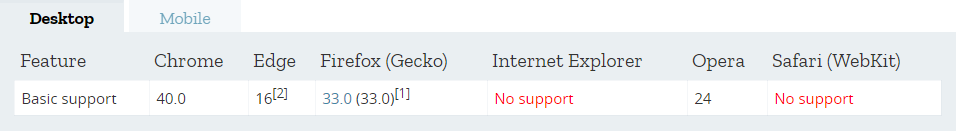
\includegraphics[width=1\linewidth]{CompWeb}
	\caption{Compatibilità web}
	\label{fig:Compatibilità web}
\end{figure}
\subsection{Mobile}
\begin{figure}
	\centering
	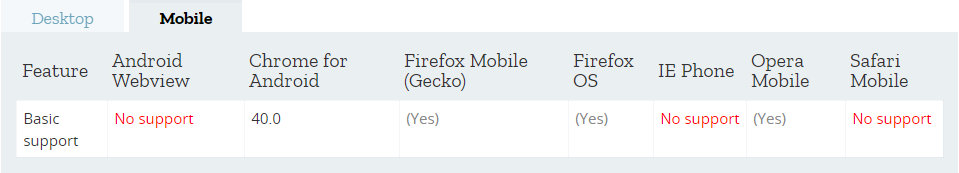
\includegraphics[width=1\linewidth]{CompMobile}
	\caption{Compatibilità mobile}
	\label{fig:Compatibilità mobile}
\end{figure}
\end{document}